\documentclass[tikz,border=5mm,12pt]{standalone}
\usetikzlibrary{positioning}

\begin{document}
  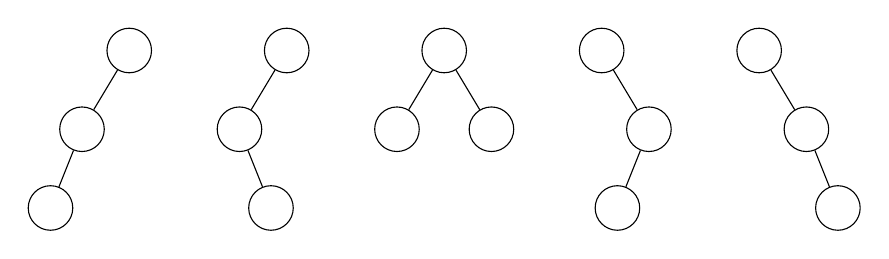
\begin{tikzpicture}[
    binarytree/.style={
      level distance=10mm,
      level 1/.style={sibling distance=12mm},
      level 2/.style={sibling distance=8mm},
      every node/.style={
        circle,draw,inner sep=2mm,anchor=center
      }
    }
  ]
    \begin{scope}[binarytree]
      \node {}
        child {node {}
          child {node {}}
          child[missing]
        }
        child[missing];
    \end{scope}

    \begin{scope}[binarytree,xshift=20mm]
      \node {}
        child {node {}
          child[missing]
          child {node {}}
        }
        child[missing];
    \end{scope}

    \begin{scope}[binarytree,xshift=40mm]
      \node {}
        child {node {}}
        child {node {}};
    \end{scope}

    \begin{scope}[binarytree,xshift=60mm]
      \node {}
        child[missing]
        child {node {}
          child {node {}}
          child[missing]
        };
    \end{scope}

    \begin{scope}[binarytree,xshift=80mm]
      \node {}
        child[missing]
        child {node {}
          child[missing]
          child {node {}}
        };
    \end{scope}
  \end{tikzpicture}
\end{document}
